% Created 2015-12-18 Fri 23:20
\documentclass[11pt]{article}
\usepackage[utf8]{inputenc}
\usepackage[T1]{fontenc}
\usepackage{fixltx2e}
\usepackage{graphicx}
\usepackage{longtable}
\usepackage{float}
\usepackage{wrapfig}
\usepackage{rotating}
\usepackage[normalem]{ulem}
\usepackage{amsmath}
\usepackage{textcomp}
\usepackage{marvosym}
\usepackage{wasysym}
\usepackage{amssymb}
\usepackage{capt-of}
\usepackage[hidelinks]{hyperref}
\tolerance=1000
\usepackage[utf8]{inputenc}
\usepackage{commath}
\usepackage{pgf}
\usepackage{tikz}
\usetikzlibrary{shapes,backgrounds}
\usepackage{marginnote}
\usepackage{listings}
\usepackage{enumerate}
\usepackage{algpseudocode}
\usepackage{algorithm}
\usepackage{mathtools}
\usetikzlibrary{arrows,automata}
\setlength{\parskip}{16pt plus 2pt minus 2pt}
\renewcommand{\arraystretch}{1.6}
\DeclareMathOperator{\Neg}{Neg}
\author{Oleg Sivokon}
\date{\textit{<2015-12-18 Fri>}}
\title{Assignment 14, Authomata Theory}
\hypersetup{
 pdfauthor={Oleg Sivokon},
 pdftitle={Assignment 14, Authomata Theory},
 pdfkeywords={Automata Theory, Formal Languages, Assignment},
 pdfsubject={Fourth assignment in the course 20440 Automata and Formal Languages},
 pdfcreator={Emacs 25.0.50.1 (Org mode 8.3beta)}, 
 pdflang={English}}
\begin{document}

\maketitle
\tableofcontents

\definecolor{codebg}{rgb}{0.96,0.99,0.8}
\definecolor{codestr}{rgb}{0.46,0.09,0.2}
\lstset{%
  backgroundcolor=\color{codebg},
  basicstyle=\ttfamily\scriptsize,
  breakatwhitespace=false,
  breaklines=false,
  captionpos=b,
  framexleftmargin=10pt,
  xleftmargin=10pt,
  framerule=0pt,
  frame=tb,
  keepspaces=true,
  keywordstyle=\color{blue},
  showspaces=false,
  showstringspaces=false,
  showtabs=false,
  stringstyle=\color{codestr},
  tabsize=2
}
\lstnewenvironment{maxima}{%
  \lstset{%
    backgroundcolor=\color{codebg},
    escapeinside={(*@}{@*)},
    aboveskip=20pt,
    captionpos=b,
    label=,
    caption=,
    showstringspaces=false,
    frame=single,
    framerule=0pt,
    basicstyle=\ttfamily\scriptsize,
    columns=fixed}}{}
}
\makeatletter
\newcommand{\verbatimfont}[1]{\renewcommand{\verbatim@font}{\ttfamily#1}}
\makeatother
\verbatimfont{\small}%
\clearpage

\section{Problems}
\label{sec:orgheadline11}

\subsection{Problem 1}
\label{sec:orgheadline4}
For each language below over the alphabet \(\Sigma = \{a, b\}\) specify the
number of equivalence classes and the distinguishing extension that
distinguishes between the said classes:

\begin{enumerate}
\item \(L = \{b, bb, bbb, bba\}\).
\item All words which begin and end in \(ba\).
\item \(L = \{c^ib^ia^i \;|\; i \geq 0\}\).
\end{enumerate}

\subsubsection{Answer 1}
\label{sec:orgheadline1}
We can distinguish between words having one character by appending
\(\epsilon\), since \(b . \epsilon\) is in the language and \(a . \epsilon\) isnt.
There are four words of length 2, namely \(aa\), \(ab\), \(ba\) and \(bb\), and we
can distinguish between \(bb\) and the rest of the words by appending
\(\epsilon\), since, again, only \(bb\) is in the language.  Finally, there are
8 words of length 3, of which \(bba\) and \(bbb\) can be distinguished from the
rest by appending \(\epsilon\).  Words of length 4 and greater are
indistinguishable since no word in \(L\) is that long.  Hence, there must
be in total 4 equivalence classes.

\subsubsection{Answer 2}
\label{sec:orgheadline2}
At first, I will define \(\delta\) for this language, thus simultaneously
showing it is regular:

\begin{center}
\begin{tabular}{lll}
 & a & b\\
\hline
\(q_0\) & \(q_f\) & \(q_1\)\\
\(q_1\) & \(q_2\) & \(q_f\)\\
\(*q_2\) & \(q_3\) & \(q_4\)\\
\(q_3\) & \(q_3\) & \(q_4\)\\
\(q_4\) & \(q_5\) & \(q_3\)\\
\(*q_5\) & \(q_3\) & \(q_4\)\\
\end{tabular}
\end{center}

Thus establishing the upper bound on number of classes: 6.  Now, I will use
a ``representative'' of every class to find the distinguishing extension.

\begin{center}
\begin{tabular}{lllll}
 & b & ba & baa & bab\\
\hline
baba & ba &  & \(\epsilon\) & a\\
bab & ba & a & a & \\
baa & ba & \(\epsilon\) &  & \\
ba & \(\epsilon\) &  &  & \\
\end{tabular}
\end{center}

Apparently, \(baba\) and \(ba\) are indistinguishable, i.e. \(q_2\) and \(q_5\)
could be unified.  Hence, the minimal automata has 5 states.  Hence,
according to Myhill-Nerode there are 5 equivalence classes.

\subsubsection{Answer 3}
\label{sec:orgheadline3}
Not only this language doesn't answer the requirement of having only two
letters in its alphabet, it is also not a regular language.  Once I prove
the language isn't regular, it immediately follows that it has infinitely
many equivalence classes.

Suppose, for contradiction, \(L\) is regular.  If this is the case, its
automaton must have a finite number of classes, say \(n\).  Now consider all
words in \(L\) starting with \(c^0\), \(c^1\) and so on trhough to \(c^n\).  In
total, there would be \(n+1\) such words, which, by pigeonhole principle
implies that at least two of them belong in the same class, i.e. must end in
the same suffix, but clearly for any two \(c^k\) and \(c^r\), where \(k \neq r\)
it is also the case that \(a^kb^k \neq a^rb^r\), hence the initial assumption
must be false.  Hence \(L\) is not regular and, consequently, has infinitely
many equivalence classes.o

\subsection{Problem 2}
\label{sec:orgheadline6}
Build the reduced DFA of the given NFA:

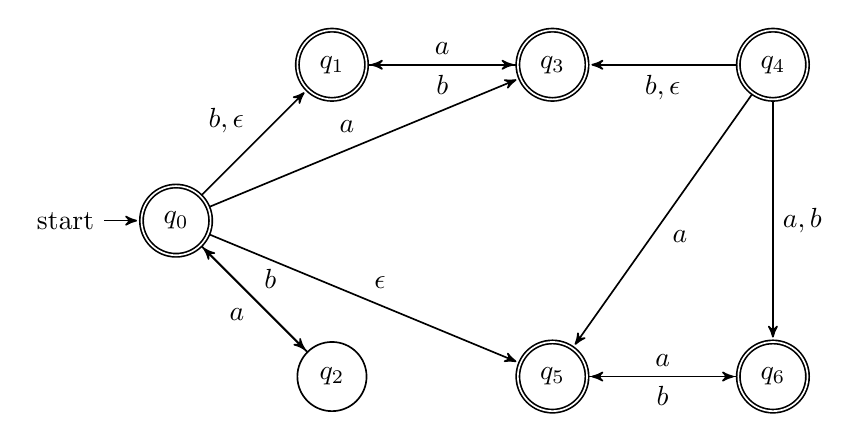
\begin{tikzpicture}[->,>=stealth',shorten >=1pt,auto,node distance=2.8cm,
                    semithick]

  \node[accepting,initial,state]   (A)              {$q_0$};
  \node[accepting,state]           (B) [above right of=A] {$q_1$};
  \node[state]                     (C) [below right of=A] {$q_2$};
  \node[accepting,state]           (D) [right of=B] {$q_3$};
  \node[accepting,state]           (E) [right of=D] {$q_4$};
  \node[accepting,state]           (F) [right of=C] {$q_5$};
  \node[accepting,state]           (G) [right of=F] {$q_6$};

  \path (A) edge              node {$b,\epsilon$} (B)
            edge              node {$a$}   (D)
            edge              node {$b$}   (C)
            edge              node {$\epsilon$} (F)
        (C) edge              node {$a$} (A)
        (B) edge              node {$a$}   (D)
        (D) edge              node {$b$}   (B)
        (E) edge              node {$b,\epsilon$} (D)
            edge              node {$a,b$} (G)
            edge              node {$a$} (F)
        (F) edge              node {$a$} (G)
        (G) edge              node {$b$} (F);
\end{tikzpicture}

\subsubsection{Answer 4}
\label{sec:orgheadline5}
In the first step, notice that there are no arrows leading to \(q_4\), this
means we can safely remove it and all the arrows leading from it:

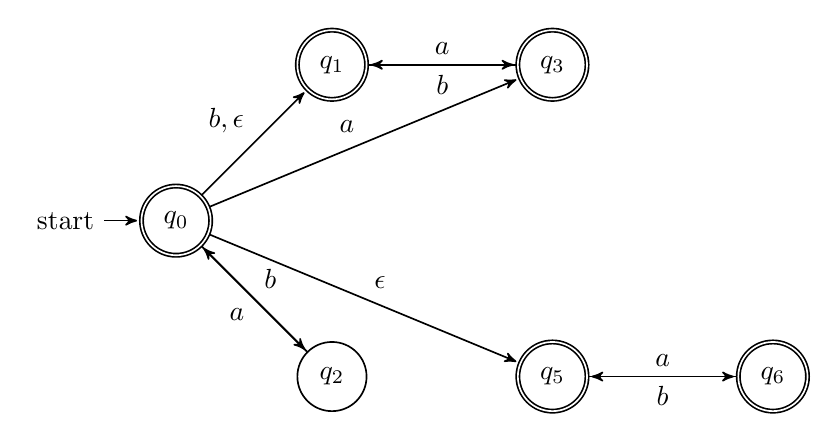
\begin{tikzpicture}[->,>=stealth',shorten >=1pt,auto,node distance=2.8cm,
                    semithick]

  \node[accepting,initial,state]   (A)              {$q_0$};
  \node[accepting,state]           (B) [above right of=A] {$q_1$};
  \node[state]                     (C) [below right of=A] {$q_2$};
  \node[accepting,state]           (D) [right of=B] {$q_3$};
  \node[accepting,state]           (F) [right of=C] {$q_5$};
  \node[accepting,state]           (G) [right of=F] {$q_6$};

  \path (A) edge              node {$b,\epsilon$} (B)
            edge              node {$a$}   (D)
            edge              node {$b$}   (C)
            edge              node {$\epsilon$} (F)
        (C) edge              node {$a$} (A)
        (B) edge              node {$a$}   (D)
        (D) edge              node {$b$}   (B)
        (F) edge              node {$a$} (G)
        (G) edge              node {$b$} (F);
\end{tikzpicture}

In the next step, we can replace all \(\epsilon\)-transitions by the arcs
leading directly to the nodes inside \(\epsilon\)-closure of the source node.

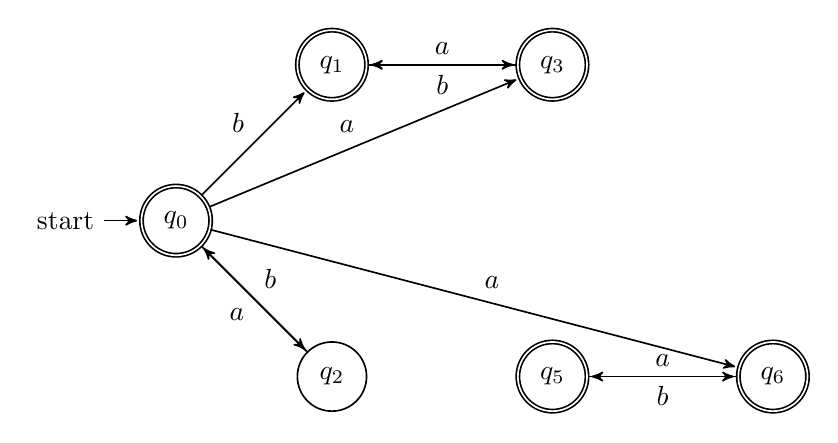
\begin{tikzpicture}[->,>=stealth',shorten >=1pt,auto,node distance=2.8cm,
                    semithick]

  \node[accepting,initial,state]   (A)              {$q_0$};
  \node[accepting,state]           (B) [above right of=A] {$q_1$};
  \node[state]                     (C) [below right of=A] {$q_2$};
  \node[accepting,state]           (D) [right of=B] {$q_3$};
  \node[accepting,state]           (F) [right of=C] {$q_5$};
  \node[accepting,state]           (G) [right of=F] {$q_6$};

  \path (A) edge              node {$b$} (B)
            edge              node {$a$} (D)
            edge              node {$b$} (C)
            edge              node {$a$} (G)
        (C) edge              node {$a$} (A)
        (B) edge              node {$a$} (D)
        (D) edge              node {$b$} (B)
        (F) edge              node {$a$} (G)
        (G) edge              node {$b$} (F);
\end{tikzpicture}

Now we can create product automation to obtain a DFA:

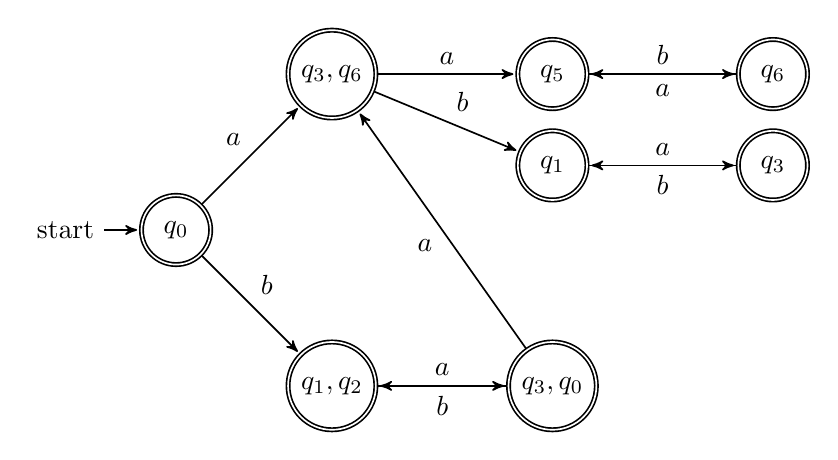
\begin{tikzpicture}[->,>=stealth',shorten >=1pt,auto,node distance=2.8cm,
                    semithick]

  \node[accepting,initial,state]   (A)              {$q_0$};
  \node[accepting,state]           (B) [above right of=A] {$q_3,q_6$};
  \node[accepting,state]           (C) [right of=B] {$q_5$};
  \node[accepting,state]           (D) [right of=C] {$q_6$};
  \node[accepting,state]           (E) [below right of=A] {$q_1,q_2$};
  \node[accepting,state]           (F) [right of=E] {$q_3,q_0$};
  \node[accepting,state]           (G) [above of=F] {$q_1$};
  \node[accepting,state]           (H) [right of=G] {$q_3$};

  \path (A) edge              node {$a$} (B)
            edge              node {$b$} (E)
        (B) edge              node {$a$} (C)
            edge              node {$b$} (G)
        (C) edge              node {$b$} (D)
        (D) edge              node {$a$} (C)
        (E) edge              node {$a$} (F)
        (F) edge              node {$a$} (B)
            edge              node {$b$} (E)
        (G) edge              node {$a$} (H)
        (H) edge              node {$b$} (G);
\end{tikzpicture}

Now we are ready to build the table of ``representatives'' of the classes:

\begin{center}
\begin{tabular}{lllllll}
 & a & b & aa & ab & ba & aab\\
\hline
aba & a & a &  & a & a & a\\
aab & b & aa & b &  & b & \\
ba & aa & b & a & b &  & \\
ab &  & aa & a &  &  & \\
aa & a & a &  &  &  & \\
b & b &  &  &  &  & \\
\end{tabular}
\end{center}

Which means that \(q_5\) and \(q_3\) can be unified, similarly \(q_1\) and \(q_6\)
and \(\{q_3,q_6\}\) with \(q_1\).  This gives us the following reduced DFA:

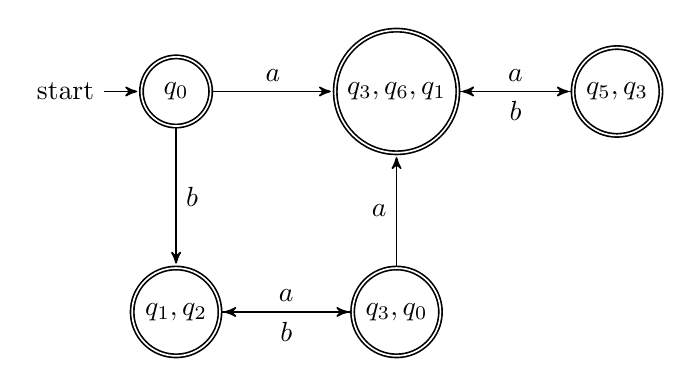
\begin{tikzpicture}[->,>=stealth',shorten >=1pt,auto,node distance=2.8cm,
                    semithick]

  \node[accepting,initial,state]   (A)              {$q_0$};
  \node[accepting,state]           (B) [right of=A] {$q_3,q_6,q_1$};
  \node[accepting,state]           (C) [right of=B] {$q_5,q_3$};
  \node[accepting,state]           (D) [below of=A] {$q_1,q_2$};
  \node[accepting,state]           (E) [right of=D] {$q_3,q_0$};

  \path (A) edge              node {$a$} (B)
            edge              node {$b$} (D)
        (B) edge              node {$a$} (C)
        (C) edge              node {$b$} (B)
        (D) edge              node {$a$} (E)
        (E) edge              node {$a$} (B)
            edge              node {$b$} (D);
\end{tikzpicture}

\subsection{Problem 3}
\label{sec:orgheadline8}
Prove that the language \(L=\{0^r1^s2^t0^{t+3} \;|\; r,s,t \geq 1\}\) is not
regular using Myhill-Nerode theorem.

\subsubsection{Answer 5}
\label{sec:orgheadline7}
Assume, for contradiction, \(L\) is regular.  Then according to Myhill-Nerode
theorem the free monoid \(\Sigma^*\) where \(\Sigma = \{0, 1, 2\}\) is
partitioned into finite number of equivalence classes by the relation \(R_L\)
defined on \(L\), where words in \(\Sigma^*\) are related iff they don't have a
distinguishing extension.  Let the number of equivalence classes created by
\(R_L\) be \(n\).  Consider the set of words where \(r=1\), \(s=1\) and \(t=1 \dots
    n + 1\).  By pigeonhole principle there must be two words in this set in the
same equivalence class.  Suppose without loss of generality \(w_1 =
    0^11^12^i\) and \(w_2 = 0^11^12^j\) where \(i \neq j\) are these words.  Then it
follows that there does not exist a distinguishing extension for them, but
if we choose \(0^{i+3}\) to be the distinguishing extension, then \(w_1\) is in
the language, but \(w_2\) isn't since \(0^{i+3} \neq 0^{j+3}\).  Hence the
initial claim is false, hence the language is not regular.

\subsection{Problem 4}
\label{sec:orgheadline10}
Given alphabet \(\Sigma\) s.t. \(\abs{\Sigma} \geq 2\) and \(1,0 \in \Sigma\), in
how many equivalence classes does the relation \(R_L\) partition its free
monoid, if the language for this relation is given by regular expression
\(\Sigma\Sigma^+10\Sigma\)?

\subsubsection{Answer 6}
\label{sec:orgheadline9}
In the first step I'll design a DFA to accept this language:

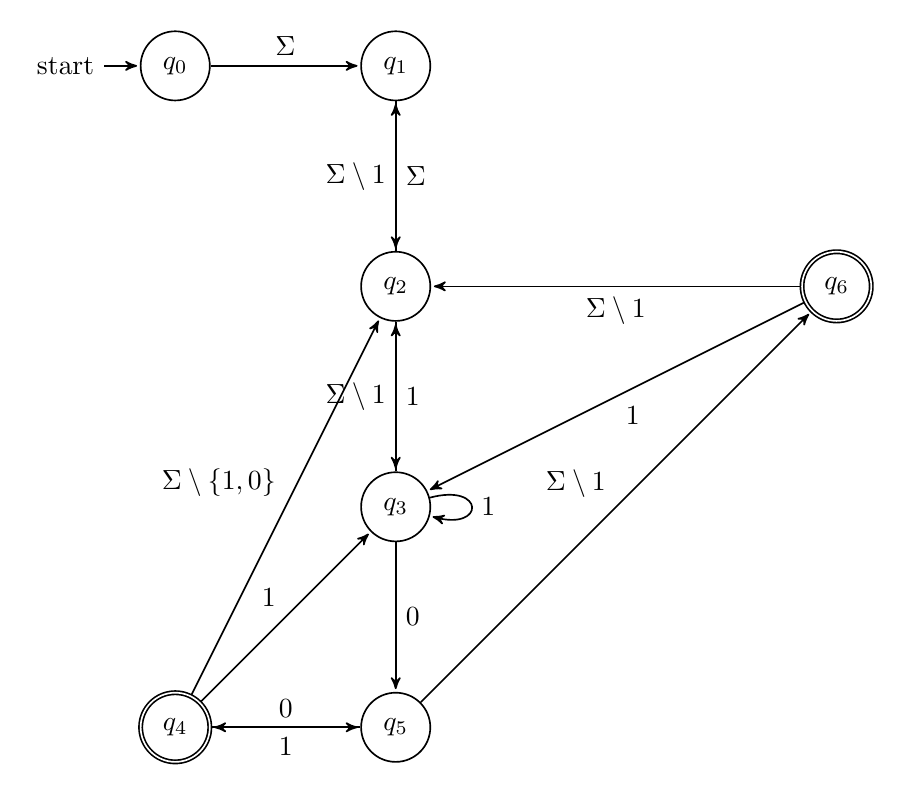
\begin{tikzpicture}[->,>=stealth',shorten >=1pt,auto,node distance=2.8cm,
                    semithick]

  \node[initial,state]   (A)              {$q_0$};
  \node[state]           (B) [right of=A] {$q_1$};
  \node[state]           (C) [below of=B] {$q_2$};
  \node[state]           (D) [below of=C] {$q_3$};
  \node[accepting,state] (E) [below of=A, left of=D] {$q_4$};
  \node[state]           (F) [below of=D] {$q_5$};
  \node[accepting,state] (G) [right of=D, right of=C] {$q_6$};

  \path (A) edge              node {$\Sigma$} (B)
        (B) edge              node {$\Sigma$} (C)
        (C) edge              node {$\Sigma \setminus 1$} (B)
            edge              node {$1$} (D)
        (D) edge              node {$0$} (F)
            edge              node {$\Sigma \setminus 1$} (C)
            edge [loop right] node {$1$} (D)
        (E) edge              node {$1$} (D)
            edge              node {$\Sigma \setminus \{1,0\}$} (C)
            edge              node {$0$} (F)
        (F) edge              node {$1$} (E)
            edge              node {$\Sigma \setminus 1$} (G)
        (G) edge              node {$1$} (D)
            edge              node {$\Sigma \setminus 1$} (C);
\end{tikzpicture}

Let's verify whether every two ``representatives'' of this automaton have a
distinguishing extension:

For the ease of notation \(\Omega = \Sigma \setminus 1\).

\begin{center}
\begin{tabular}{lrrrl}
 & \(\Sigma\) & \(\Sigma\Sigma\) & \(\Sigma\Sigma 1\) & \(\Sigma\Sigma 10\)\\
\hline
\(\Sigma\Sigma 10\Omega\) & \(\epsilon\) & \(\epsilon\) & \(\epsilon\) & \(\epsilon\)\\
\(\Sigma\Sigma 10\) & 1 & 1 & 1 & \\
\(\Sigma\Sigma 1\) & 0 & 0 &  & \\
\(\Sigma\Sigma\) & 101 &  &  & \\
\end{tabular}
\end{center}

Since we could find a distinguishing extension for each pair of the states
in the automaton, it follows that the number of equivalence classes is the
same as the number of the states, i.e. 7.
\end{document}